% !TeX root = ../note.tex
\sectioncentered*{Перечень условных обозначений, символов и терминов}\label{sec:definitions}
\addcontentsline{toc}{section}{Перечень условных обозначений, символов и терминов}\label{sec:introduction}
\pagenumbering{arabic}
\setcounter{page}{6}

В настоящей пояснительной записке применяются следующие определения и сокращения.
\\

\emph{Спецификация} — документ, который желательно полно, точно и верифицируемо определяет требования, дизайн, поведение или другие характеристики компонента или системы, и, часто, инструкции для контроля выполнения этих требований~\cite{istqb_specification}.

\emph{Сервис\hyphориентированная архитектура} — модульный подход к разработке программного обеспечения, основанный на использовании распределённых, слабо связанных заменяемых компонентов, оснащённых стандартизированными интерфейсами для взаимодействия по стандартизированным протоколам~\cite{wiki_soa}.

\emph{Горизонтальное масштабирование} — разбиение системы на более мелкие структурные компоненты и разнесение их по отдельным физическим машинам (или их группам), и (или) увеличение количества серверов, параллельно выполняющих одну и ту же функцию.

ПС — программное средство.

ПО — программное обеспечение.

БД — база данных.

СУБД — система управления базами данных.

API — Application Programming Interface (программный интерфейс приложения).

HTTP - HyperText Transfer Protocol.

JSON — JavaScript Object Notation (текстовый формат обмена данными, основанный на JavaScript).

XML - eXtensible Markup Language (формат сериализации данных и язык разметки).

UI — user interface (пользовательский интерфейс).

JWT — JSON Web Token.

ТЭО — технико-экономическое обоснование.

\newpage

\sectioncentered*{Введение}
\addcontentsline{toc}{section}{Введение}\label{sec:introduction}

В современном мире индустрия разработки программного обеспечения очень велика. Процесс разработки всё время становится сложнее и дороже, что негативно сказывается на развитии индустрии в целом. Не лучшим образом на ситуацию влияют дефицит высококвалифицированных специалистов в сфере информационных технологий. В современной ситуации компании всё чаще занимаются не только подбором персонала, но и содействием в развитии сотрудником. Развитие персонала рассматривается как особый вид инвестиции, который позволяет увеличить производительности труда и рентабельность бизнеса, сократить производственные и экономические потери, связанные с влиянием человеческого фактора.

Одним из способов повышения эффективности и продуктивности разработки является внедрение систем отслеживания ошибок и развития персонала.

Система отслеживания ошибок — прикладная программа, разработанная с целью помочь разработчикам программного обеспечения учитывать и контролировать ошибки и неполадки, найденные в программах, пожелания пользователей, а также следить за процессом устранения этих ошибок и выполнения или невыполнения пожеланий.

Главным компонентом системы отслеживания ошибок – база данных, которая содержит в себе сведения об обнаруженных дефектах. Обычно эти сведения содержат в себе:
\begin{itemize}
    \item номер (идентификатор) дефекта;
    \item короткое описание дефекта;
    \item кто сообщил о дефекте;
    \item дата и время, когда был обнаружен дефект;
    \item версия продукта, в которой обнаружен дефект;
    \item серьёзность (критичность) дефекта и приоритет решения;
    \item описание шагов для выявления дефекта (воспроизведения непреднамеренного поведения программы);
    \item ожидаемый результат и фактический результат;
    \item кто ответственен за устранение дефекта;
    \item обсуждение возможных решений и их последствий;
    \item текущее состояние (статус) дефекта.
\end{itemize}

Система отслеживания ошибок является необходимым компонентом инфраструктуры профессиональной разработки программного обеспечения. Её использование считается одним из отличительных признаков хорошей команды разработчиков программного обеспечения, так как увеличивает производительность программистов, систематизирует и автоматизирует борьбу с ошибками.

Система развития персонала - это прикладная программа, разработанная для эффективного выполнения текущих и перспективных производственных задач, а также оптимального удовлетворения запросов работников, связанных с самореализацией, профессиональной подготовкой и карьерой. 

Интеграция системы развития сотрудников также положительно сказывается на эффективности и ценности программиста как специалиста благодаря постоянной постановке перед собой новых задач в изучении новых технологий или направлений. Выполняя данные задачи, программист увеличивает свой теоретический и практический опыт.

В данном дипломном проекте реализуется программное средство для для развития сотрудников и управления проектами. Данное ПС предоставляет функционал для работы с информацией об организации, её сотрудниках и менеджерах, позволяет ставить цели в развитии и изучении новых технологий, организовывать прозрачную работу над проектами, реализовывать авторизацию и аутентификацию пользователей.

В рамках дипломного проекта реализуется несколько независимых сервисов, связанных друг с другом. Сервисы включают в себя:
\begin{itemize}
    \item employee development service — сервис, предоставляющий функционал для развития персонала;
    \item project management service - сервис, позволяющий организовывать работу над проектами;
    \item file service — сервис, хранящий загруженные пользователями файлы;
    \item notification service - сервис, который посылает уведомления пользователям о различных событиях;
    \item authority service — сервис, который хранит авторизационные данные пользователей и обеспечивает идентификацию пользователя.
\end{itemize}

В пояснительной записке к дипломному проекту излагаются детали поэтапной разработки веб-приложения для развития персонала и управления проектами. В первом разделе приведены результаты анализа литературных источников по теме дипломного проекта, рассмотрены особенности существующих систем-ана\-логов, выдвинуты требования к проектируемому ПС. Во втором разделе проводится моделирование предметной области, описываются сервисы, которые необходимо разработать, описываются функциональные требования к модулям, включенным в сервисы, а также нефункциональные требования к разработке проекта. Также в разделе описаны модели данных, которые должны использоваться в сервисах. В третьем разделе приводятся описания используемых технологий, таких как базы данных, языка программирования и технологий для передачи данных между сервисами. В четвертом разделе представлены доказательства того, что сервисы разработаны в соответствии с выдвинутыми требованиями, приведены фрагменты кода, демострирующие детали реализации проекта. В пятом разделе приведены сведения по развёртывания и запуску программного средства, указаны требуемые программные средства. Обоснование и целесообразность создания программного средства с технико-экономической точки зрения приведено в шестом разделе. Итоги проектирования, конструирования программного средства, а также соответствующие выводы приведены в заключении.

Дипломный проект проверен в системе «Антиплагиат» (рисунок~\ref{fig:antiplagiat}). Процент оригинальности соответствует норме, установленной кафедрой информатики. Цитирования обозначены ссылками на публикации, указанные в «Списке использованных источников».

\begin{figure}[ht]
    \centering
    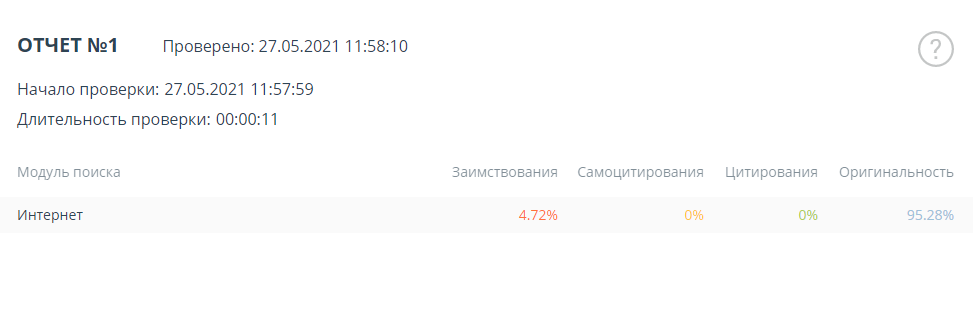
\includegraphics[width=\textwidth]{antiplagiat}
    \renewcommand{\thefigure}{1}
    \caption{Скриншот проверки диплома в системе «Антиплагиат»}\label{fig:antiplagiat}
\end{figure}